\documentclass[twoside]{article}
\usepackage{microtype, fontspec}
\usepackage{textcomp, gensymb, amsmath, mathtools, siunitx, unicode-math}
% Page layout
\usepackage[a4paper, margin=20mm, headheight=12.0pt]{geometry}
\usepackage{fancyhdr, multicol, graphicx, caption, tabu, longtable, float, booktabs, tabularx, listings, xcolor, pdfpages, subcaption, titling, titlesec, enumitem, url, currency, pdflscape}
\usepackage[toc,page]{appendix}
\usepackage[style=ieee, backend=biber]{biblatex}
\usepackage[thinc]{esdiff}
\usepackage[colorlinks=true, linkcolor=blue, citecolor=red]{hyperref}

% Typefaces
\setmonofont{Iosevka SS15}
% \setmainfont{IBM Plex Sans}
\setmainfont{Latin Modern Sans}
% \setmonofont{Cascadia Code}
\setmathfont{Latin Modern Math}

% Maths formatting
\newcommand\ddfrac[2]{\frac{\displaystyle #1}{\displaystyle #2}}

% Colors
\definecolor{listingblue}{HTML}{2196f3}
\definecolor{blue}{HTML}{0069c0}
\definecolor{grey}{HTML}{9e9e9e}

% siunitx unit shortening
\newcommand{\amp}{\ampere}
\newcommand{\m}{\metre}
\DeclareSIUnit\vpp{\text{\ensuremath{V_{\textup{p-p}}}}}
\DeclareSIUnit\voltdc{\text{\ensuremath{VDC}}}

% Currency
\DefineCurrency{USD}{name={dollar}, plural={dollars}, symbol={\$}, iso={USD}, kind=iso, base=2, cents=true, pre=true}

% Figure
\newenvironment{Figure}
    {\par\medskip\noindent\minipage{\linewidth}}
    {\endminipage\par\medskip}

% Table formatting
\renewcommand{\arraystretch}{1.5}
\setlength{\tabcolsep}{5pt}
% \captionsetup[table]{skip=0pt}

% Bibliography
\addbibresource{TermThreeProject.bib}
\nocite{*}

% Header and footer
% Title page
\fancypagestyle{plain}{
    \fancyhf{}
    \fancyhead{}
    \fancyfoot[RO,LE]{\thepage}
    \renewcommand{\headrulewidth}{0pt}
}

% Normal pages
\pagestyle{fancy}
\fancyhf{}
\fancyhead{}
\fancyfoot[R]{\thepage}
\fancyfoot[L]{}
\renewcommand{\headrulewidth}{0pt}
\pagenumbering{roman}

% Start Document
\begin{document}

% Cover Sheet

% Title Page
\begin{titlingpage}
    {\centering
    \vspace*{3cm}
    {\LARGE\textbf{Arduino Shield HeadLight}\\}
    \vspace{1cm}
    {\textbf{Edward Manson (75953196)}\\}
    {\textbf{Alex Stiles (18120890)}\\}
    \vspace{1cm}
    {\today}
    \vfill
    \noindent
    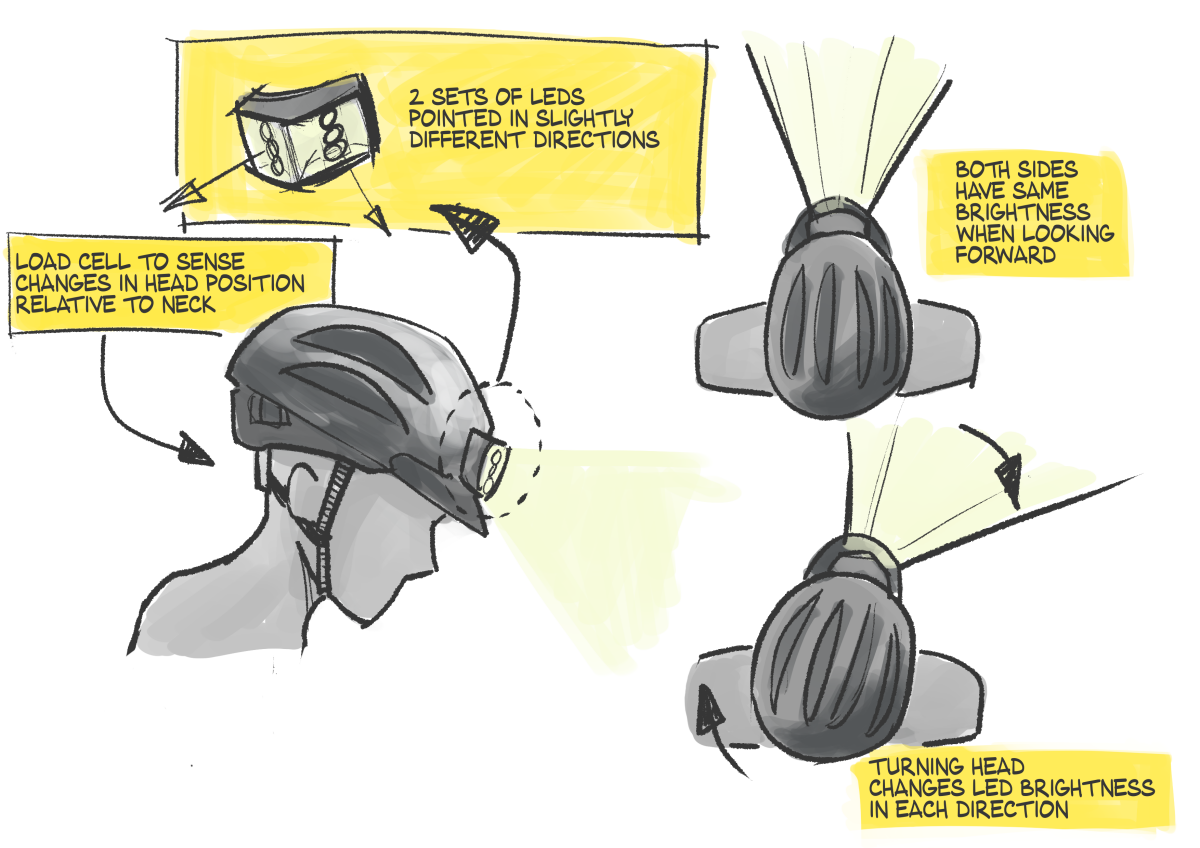
\includegraphics[width=0.75\linewidth]{headlamp-project-concept.png}
    \vfill}
\end{titlingpage}

% ToC

{\hypersetup{linkcolor=black}
\tableofcontents
\listoffigures
\listoftables
\lstlistoflistings}
\newpage

% Update Footer
\pagenumbering{arabic}
\fancyhead[C]{ENEL200}
\fancyhead[RE,LO]{Arduino Shield HeadLight}
\fancyfoot[C]{Edward Manson \& Alex Stiles}

\section{Introduction}

\section{Background}
    \noindent
    \begin{figure}[H]
        \centering
        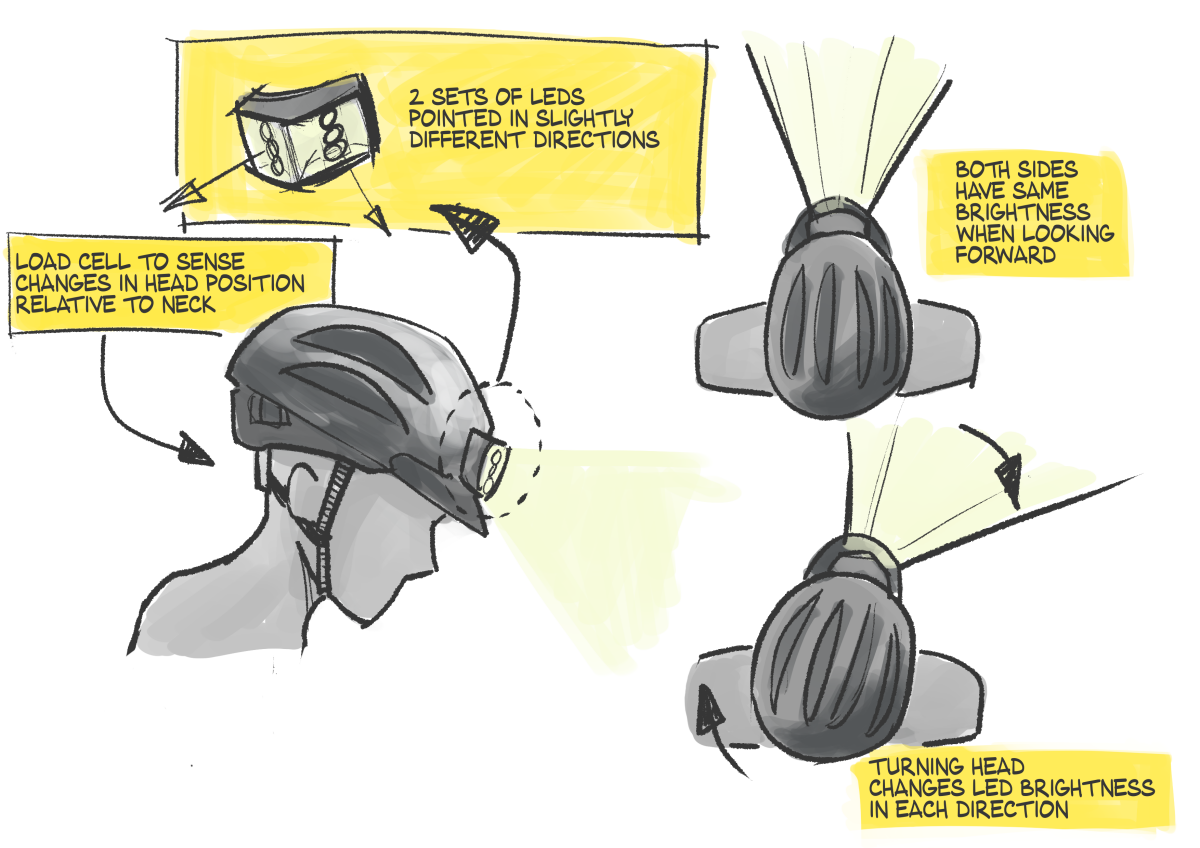
\includegraphics[width=0.75\textwidth]{headlamp-project-concept.png}
        \caption{A sketch of the HeadLight}
        \label{fig:sketch}
    \end{figure}

\section{Requirements \& Specifications}
    \subsection{Requirements}
    \subsection{Specifications}

\section{Design Overview \& Rationale}
    \subsection{Arduino Shield}
        \paragraph{}
        A load cell is used to measure the force of the head rotation, which has an internal Wheatstone bridge. The output from the Wheatstone bridge goes into an instrumentation amplifier. The instrumentation amplifier consists of non-inverting amplifiers on the output of the Wheatstone bridge, which then goes into a differential amplifier, as shown in figure \ref{fig:inamp}. The output of the differential amplifier goes into an LC low pass filter to remove high-frequency noise.
        \noindent
        \begin{figure}[H]
            \centering
            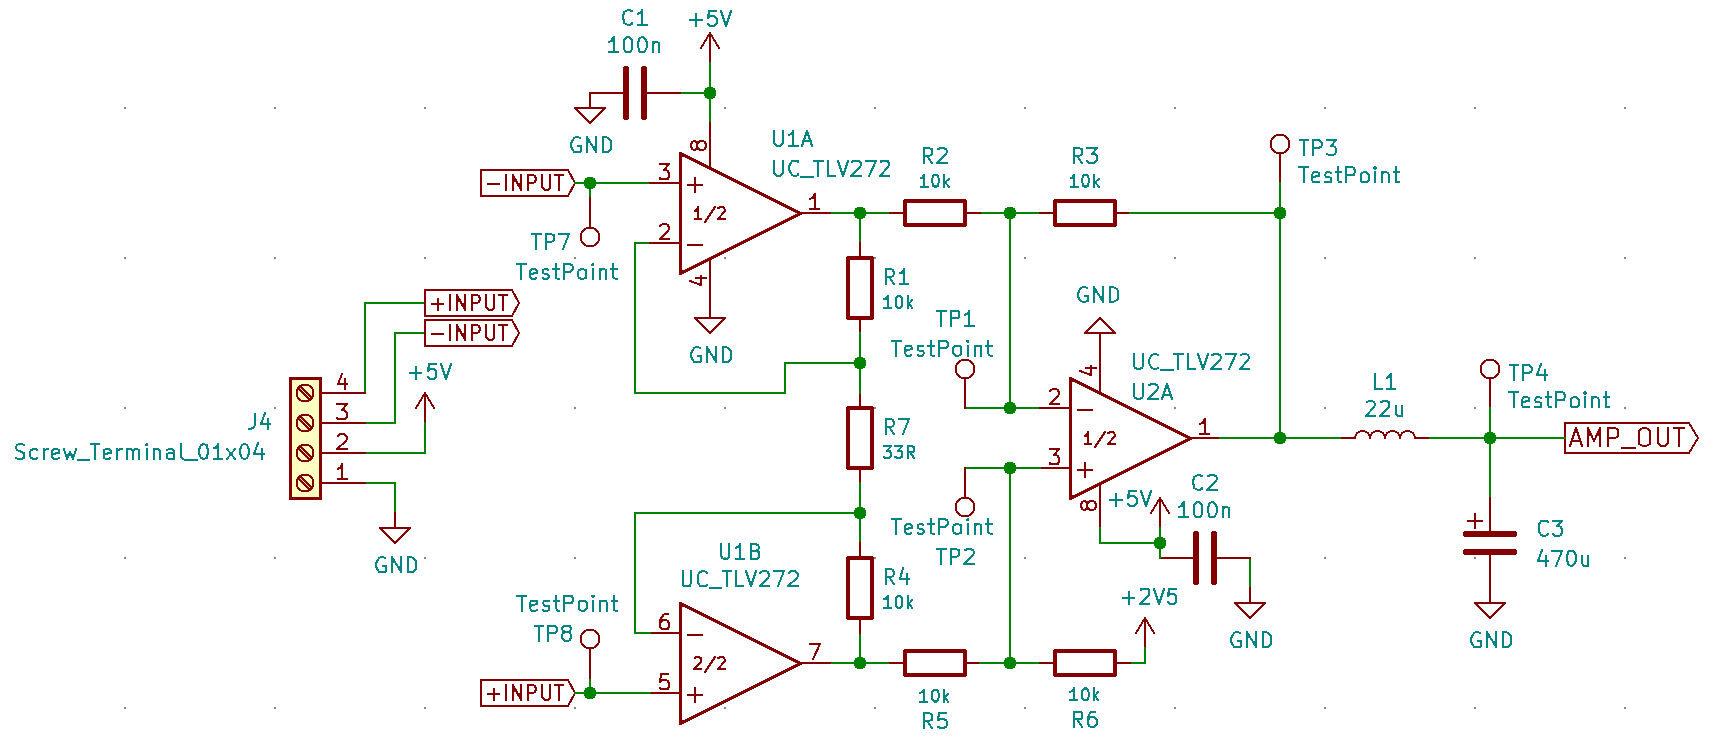
\includegraphics[width=\textwidth]{inamp.png}
            \caption{The layout of the instrumentation amplifier.}
            \label{fig:inamp}
        \end{figure}
        The output of the differential amplifier can end up being a negative value, as the Arduino can not read negative voltage, and there is no negative supply for the differential amplifier; the differential amplifier has to be biased. A voltage reference was constructed out of a voltage divider of equal values and a buffer to bias the instrumentation amplifier (shown in figure \ref{fig:vref}).
        \noindent
        \begin{figure}[H]
            \centering
            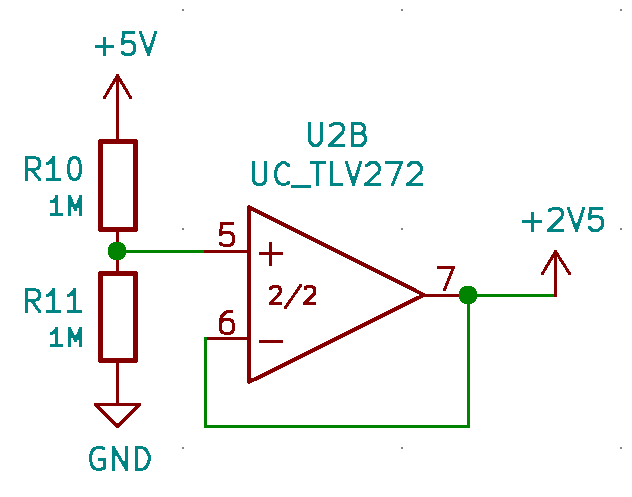
\includegraphics[width=0.75\textwidth]{vref.png}
            \caption{The layout of the voltage reference.}
            \label{fig:vref}
        \end{figure}
        For each LED array, the PWM output from the Arduino goes into the gate of a MOSFET. The current limiting resistor is connected to the anode of the LEDs, and the cathode of the LEDs is connected to the drain of the MOSFET.
        \noindent
        \begin{figure}[H]
            \centering
            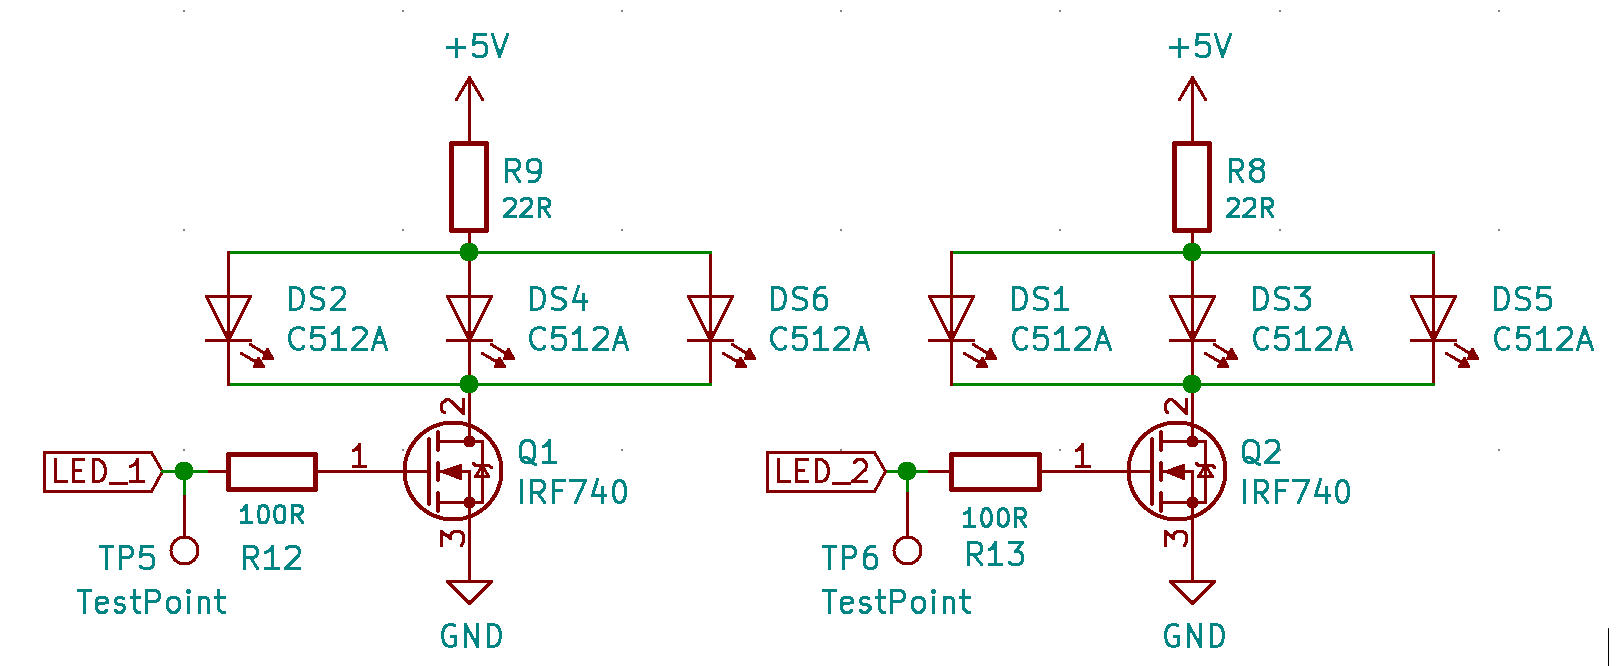
\includegraphics[width=0.75\textwidth]{ledarray.png}
            \caption{The layout of the LED arrays.}
            \label{fig:led}
        \end{figure}

        \subsubsection{PCB Layout}
        \paragraph{}
        The PCB was laid out to ensure that the ground plane would have no cuts, maximising EMC performance. Decoupling capacitors were placed right next to the power pins of the ICs. Additional care was taken so that traces were not too close to any antipads, as having traces too close to antipads can worsen EMC \cite{emc}. Test points were added so that we can troubleshoot any problems when assembling the prototype. 1x1 header were used as ground test points so that the ground clip of the oscilloscope probe can be attached.

        \subsubsection{Amplifier}
        \paragraph{}
        An instrumentation amplifier was chosen to amplify the signal from the load cell. The instrumentation amplifier consists of two non-inverting amplifiers, of which the outputs go into a differential amplifier. As the Arduino cannot read negative voltages, nor is there a negative supply, the differential amplifier was biased with \SI{2.5}{\volt}. This results in the positive difference being between \SI{2.5}{\volt} and \SI{5}{\volt}, and the negative difference is between \SI{0}{\volt} and \SI{2.5}{\volt}. A one op-amp differential amplifier has an extremely low input impedance; thus the Wheatstone bridge must have a matched impedance. A two op-amp instrumentation amplifier would require one less package but would be less stable than the three op-amp instrumentation amplifier. The three op-amp instrumentation amplifier also has a spare op-amp which is then utilised for the voltage reference.

        An initial gain of \SI{24}{\ohm} was calculated (as shown in equation \eqref{eq:g4}) \cite{ti:sloa034}, but after some test on a breadboard, the gain was changed \SI{33}{\ohm}. This was partly due to the load cell to measure \SI{\sim 50}{\percent} more than rated \cite{htc:tal221}.
        \begin{align}
            V_{O} &= \left[ \left(\text{Sig}^{+}\right) - \left(\text{Sig}^{-}\right)\right]\left[\frac{R_{4}}{R_{2}} \left[\frac{2R_{f}}{R_{g}} + 1\right] \right] \label{eq:g1}\\
            R_{g} &= \ddfrac{2R_{f}}{\left[\frac{V_{O}}{\left(\text{Sig}^{+}\right) - \left(\text{Sig}^{-}\right)} \frac{R_{2}}{R_{4}} \right]-1} \label{eq:g2}\\
            &= \ddfrac{2 \cdot \SI{10}{\kilo\ohm}}{\left[\frac{\SI{2.5}{\volt}}{\SI{3}{\milli\volt}} \frac{\SI{10}{\kilo\ohm}}{\SI{10}{\kilo\ohm}} \right]-1} \label{eq:g3}\\
            &= \SI{24.03}{\ohm} \label{eq:g4}
        \end{align}

        \subsubsection{Voltage reference}
        \paragraph{}
        A voltage divider was used to produce \SI{2.5}{\volt} to bias the differential amplifier. It was decided to use a buffer on the output of the voltage divider so that the common-mode rejection error is minimised. This is due to the op-amp's low output impedance, which does not introduce any noticeable common-mode rejection error. A \SI{2.5}{\volt} Zener diode would have been preferred. The resistors in the voltage divider have tolerances and therefore may not give exactly \SI{2.5}{\volt}; however, \SI{2.5}{\volt} Zener diodes were not available from the store. \SI{1}{\mega\ohm} resistors were chosen to limit the current and thus power consumption.

        \subsubsection{Filter}
        \paragraph{}
        A filter was used to filter out high-frequency noise from the load cell. The filter was chosen to be an LC filter. An RC filter could have been used, but it would have caused the signal's voltage to drop slightly due to the voltage drop across the resistor. The LC filter does require more space on the PCB, but the PCB had enough room for the capacitor and the inductor. LC filters also have better attenuation as the attenuation slope is twice as steep as an RC filter. The filter was placed on the output of the differential amplifier. If filters were placed on the inputs of the differential op-amp, more components would be needed, and there would not be enough space on the board. A \SI{22}{\micro\henry} inductor was chosen due to its availability in the electronics store. A \SI{470}{\micro\farad} capacitor was selected as a compromise of its physical size, cutoff frequency, and availability. The cutoff frequency was found to be \SI{1.595}{\kilo\hertz}, as shown below:
        \begin{align}
            f &= \ddfrac{1}{2 \pi \sqrt{L C}} \label{eq:f1}\\
            &= \ddfrac{1}{2 \pi \sqrt{\SI{22}{\micro\henry} \SI{470}{\micro\farad}}} \label{eq:f2}\\
            &= \SI{1.595}{\kilo\hertz} \label{eq:f3}
        \end{align}

        \subsubsection{LED arrays}
        \paragraph{}
        Each LED array has a MOSFET; this was done to have enough current supplied to the LEDs. The pins that can output PWM are only able to supply \SI{40}{\milli\amp}, so the outputs from these pins were connected to the gates of the MOSFETs. This allows the LEDs to take full current and are thus brighter. IRF740 MOSFETs were chosen due to their availability in the store and their low resistance. They have a max current of 10 A, so more LEDs can be added if required. The low resistance of the IRF740 (\SI{0.55}{\ohm}), reduces the power losses when the MOSFET is on. Individual resistors could have been matched to each LED; however, this would increase the number of components and take up extra space on the PCB. \SI{100}{\ohm} resistors were placed between the PWM output from the Arduino and the gate of the MOSFETs, this was done to minimise ringing and to limit current.

\section{Testing}
    The PCB will be assembled and attached to an Arduino. The code will be uploaded to the Arduino. The load cell will be manipulated, and the PWM signal will be probed using an oscilloscope. The duty cycle of the PWM signal will be compared to the expected duty cycle.
    The LEDs will then be connected, and the load cell manipulated to check that the LEDs behave as expected in terms of brightness and direction changes. 

\section{Conclusions}
\newpage
% Bibliography
\printbibliography

\newpage
\begin{appendices}
    \section{Applications of the Design Toolkit}
        \begin{table}[h]
            \centering
            \caption{Applications of the Design Toolkit.} \label{table:designtoolkit}
            \begin{tabularx}{\linewidth}{l l X}
                \toprule
                Tool Type & Tool Name & Where/How Used \\
                \midrule
                Strategy & Divide \& Conquer & Divide and conquer was used to split up the hardware design into:
                \begin{itemize}
                    \item Instrumentation amplifier
                    \item LED arrays and driver
                    \item \SI{2.5}{\volt} reference
                    \item LC filter
                \end{itemize}  \\
                Building Block & Amplifier & An instrumentation amplifier was constructed out of operational amplifiers to appropriately amplify the signal from the Wheatstone bridge in the load cell. \\
                Building Block & LC Filter & An LC filter was used to filter out noise from the load cell, and to not attenuate the signal. \\
                Building Block & Buffer & A buffer was used to create a low impedance voltage reference. \\
                Building Block & Current Limiting Resistor & Current limiting resistors were usd to limit the gate current for the MOSFETs and the current through the LEDs. \\
                Building Block & Arduino microcontroller &  \\
                Building Block & Pull up resistor &  \\
                Building Block & Analog input &  \\
                Building Block & Digital output &  \\
                % Building Block & 
                \bottomrule
            \end{tabularx}
        \end{table}
    \newpage
    \section{Code}
        \label{appendix:listing}
        \lstset{language=C++,
                basicstyle=\small\ttfamily,
                numberstyle=\ttfamily,
                numbers=left,
                breaklines=true,
                tabsize=4,
                keywordstyle=\color{listingblue},
                commentstyle=\color{grey},
                caption=Button code.,
                label=Listing:1,
                captionpos=b
        }
        \lstinputlisting{../main/button.c}
        \lstset{language=C++,
                basicstyle=\small\ttfamily,
                numberstyle=\ttfamily,
                numbers=left,
                breaklines=true,
                tabsize=4,
                keywordstyle=\color{listingblue},
                commentstyle=\color{grey},
                caption=Button header code.,
                label=Listing:1,
                captionpos=b
        }
        \lstinputlisting{../main/button.h}
        \lstset{language=C++,
                basicstyle=\small\ttfamily,
                numberstyle=\ttfamily,
                numbers=left,
                breaklines=true,
                tabsize=4,
                keywordstyle=\color{listingblue},
                commentstyle=\color{grey},
                caption=LED group code.,
                label=Listing:1,
                captionpos=b
        }
        \lstinputlisting{../main/LED_Group.c}
        \lstset{language=C++,
                basicstyle=\small\ttfamily,
                numberstyle=\ttfamily,
                numbers=left,
                breaklines=true,
                tabsize=4,
                keywordstyle=\color{listingblue},
                commentstyle=\color{grey},
                caption=LED group header code.,
                label=Listing:1,
                captionpos=b
        }
        \lstinputlisting{../main/LED_Group.h}
        \lstset{language=C++,
                basicstyle=\small\ttfamily,
                numberstyle=\ttfamily,
                numbers=left,
                breaklines=true,
                tabsize=4,
                keywordstyle=\color{listingblue},
                commentstyle=\color{grey},
                caption=LED group collection code.,
                label=Listing:1,
                captionpos=b
        }
        \lstinputlisting{../main/LED_Group_Collection.c}
        \lstset{language=C++,
                basicstyle=\small\ttfamily,
                numberstyle=\ttfamily,
                numbers=left,
                breaklines=true,
                tabsize=4,
                keywordstyle=\color{listingblue},
                commentstyle=\color{grey},
                caption=LED group collection header code.,
                label=Listing:1,
                captionpos=b
        }
        \lstinputlisting{../main/LED_Group_Collection.h}
        \lstset{language=C++,
                basicstyle=\small\ttfamily,
                numberstyle=\ttfamily,
                numbers=left,
                breaklines=true,
                tabsize=4,
                keywordstyle=\color{listingblue},
                commentstyle=\color{grey},
                caption=Load cell code.,
                label=Listing:1,
                captionpos=b
        }
        \lstinputlisting{../main/Load_Cell.c}
        \lstset{language=C++,
                basicstyle=\small\ttfamily,
                numberstyle=\ttfamily,
                numbers=left,
                breaklines=true,
                tabsize=4,
                keywordstyle=\color{listingblue},
                commentstyle=\color{grey},
                caption=Load cell header code.,
                label=Listing:1,
                captionpos=b
        }
        \lstinputlisting{../main/Load_Cell.h}
        \lstset{language=C++,
                basicstyle=\small\ttfamily,
                numberstyle=\ttfamily,
                numbers=left,
                breaklines=true,
                tabsize=4,
                keywordstyle=\color{listingblue},
                commentstyle=\color{grey},
                caption=Main code.,
                label=Listing:1,
                captionpos=b
        }
        \lstinputlisting{../main/main.c}
        \lstset{language=C++,
                basicstyle=\small\ttfamily,
                numberstyle=\ttfamily,
                numbers=left,
                breaklines=true,
                tabsize=4,
                keywordstyle=\color{listingblue},
                commentstyle=\color{grey},
                caption=Voltage ADC code.,
                label=Listing:1,
                captionpos=b
        }
        \lstinputlisting{../main/voltage.c}
        \lstset{language=C++,
                basicstyle=\small\ttfamily,
                numberstyle=\ttfamily,
                numbers=left,
                breaklines=true,
                tabsize=4,
                keywordstyle=\color{listingblue},
                commentstyle=\color{grey},
                caption=Voltage ADC header code.,
                label=Listing:1,
                captionpos=b
        }
        \lstinputlisting{../main/voltage.h}
        \lstset{language=C++,
                basicstyle=\small\ttfamily,
                numberstyle=\ttfamily,
                numbers=left,
                breaklines=true,
                tabsize=4,
                keywordstyle=\color{listingblue},
                commentstyle=\color{grey},
                caption=Main code.,
                label=Listing:1,
                captionpos=b
        }
        \lstinputlisting{../main/main.ino}
    \newpage
    \section{Schematic}
        \label{appendix:schematic}
        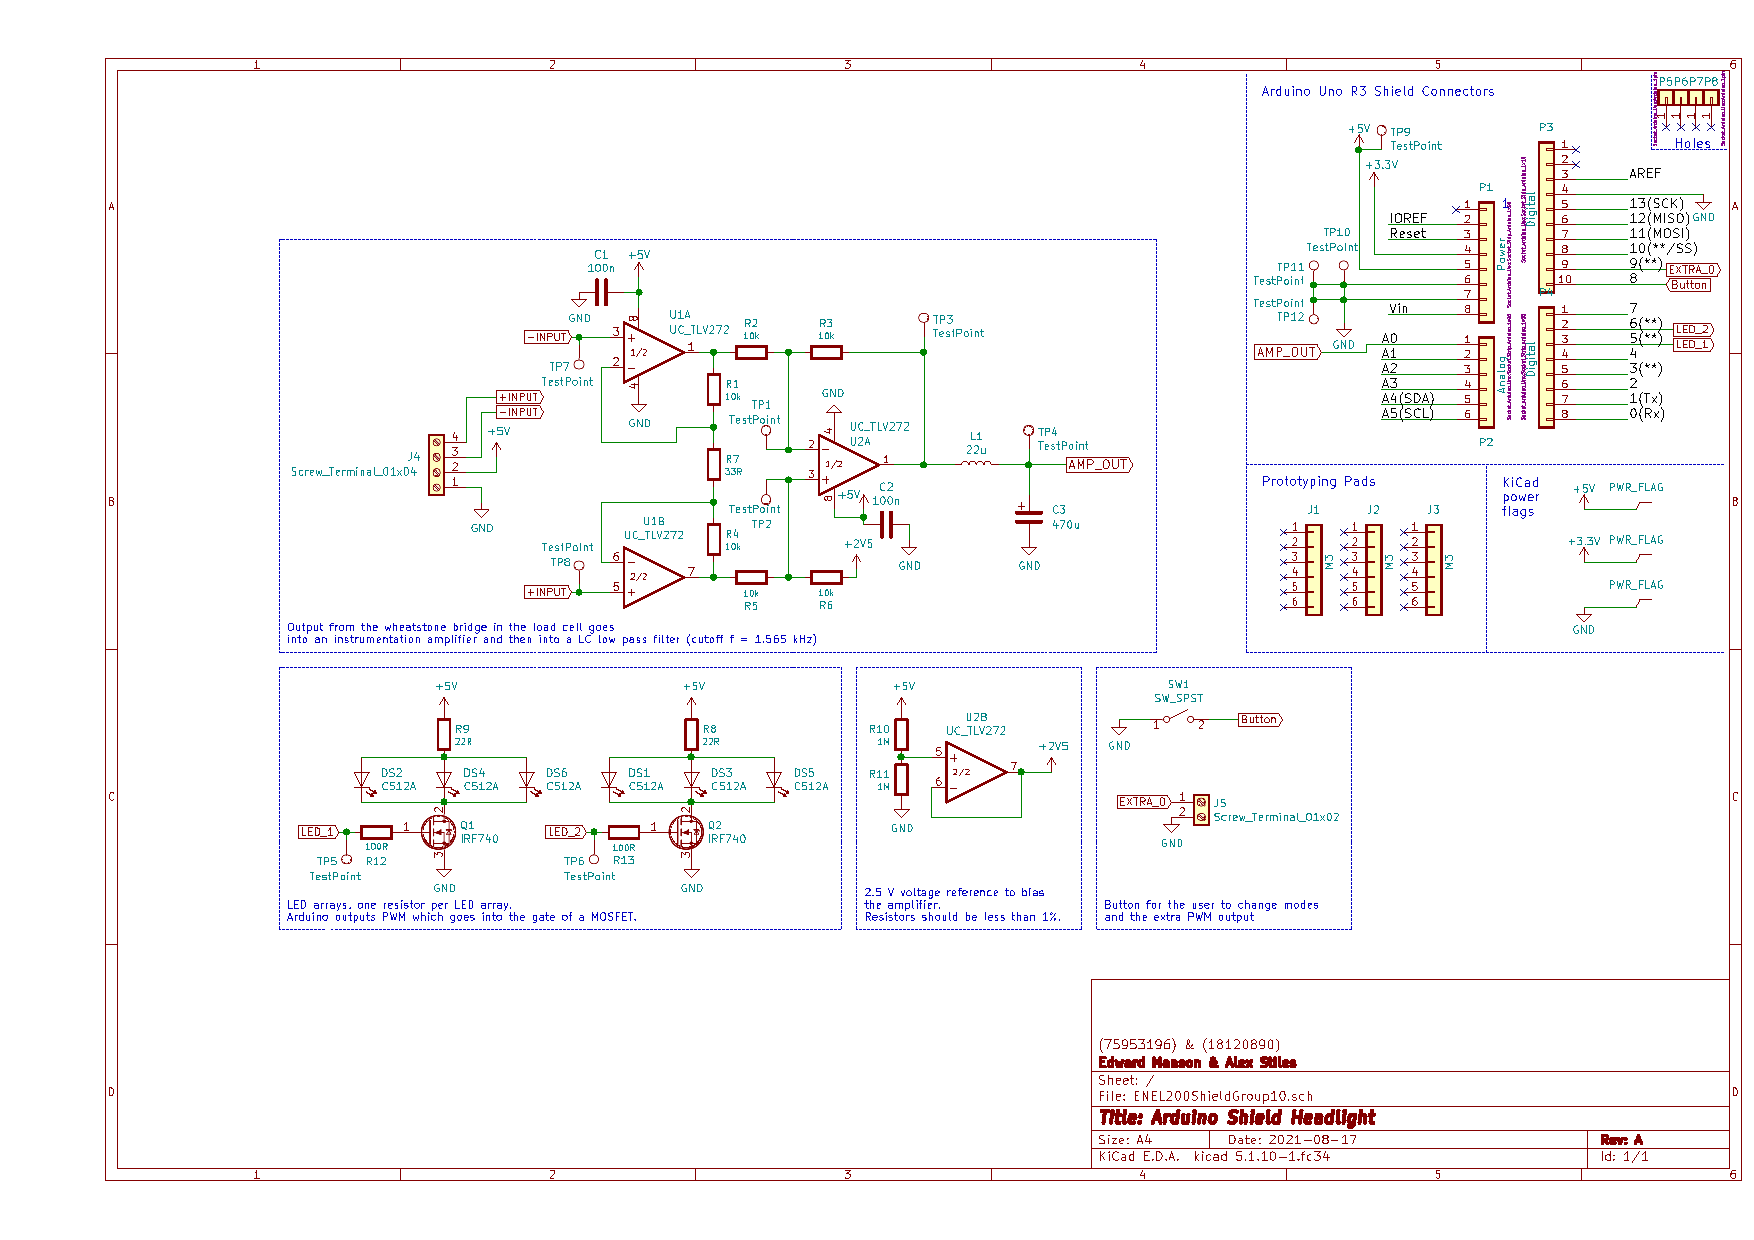
\includepdf[pages=-,landscape=true]{schematic.pdf}
    \newpage
    \section{Printed Circuit Board}
        \label{appendix:pcb}
        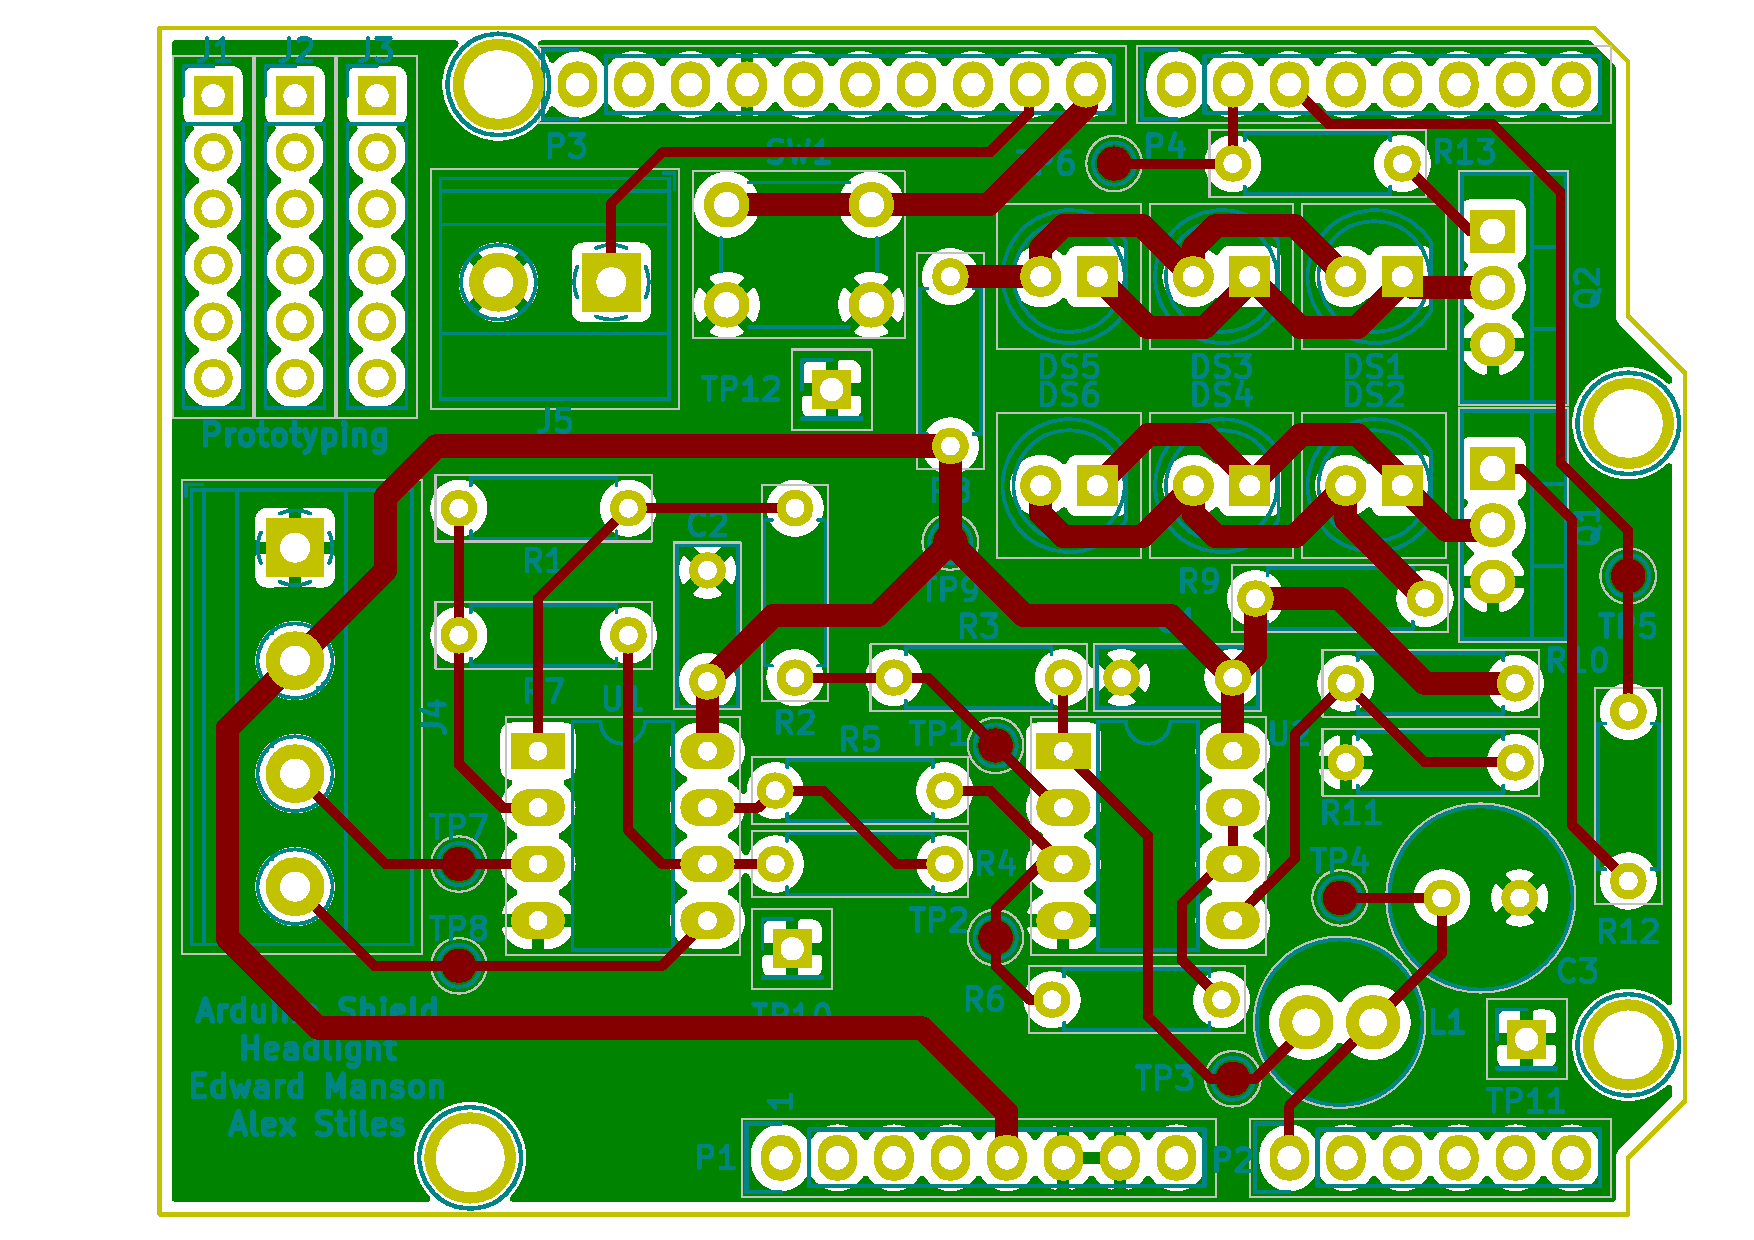
\includepdf[pages=-,landscape=true]{pcb.pdf}
    % \newpage
    % \section{Bill of Materials}
    %     \label{appendix:BOM}
    %     \noindent
    %     \begin{table}[H]
    %         \centering
    %         \begin{tabular}{ p{2.5cm} c l p{5cm} S }
    %             \toprule
                % Ref. & Qnty & Value & Description & {Price (individual per 100)} \\
                % & & & & {(\cUSD)}\\
                % \midrule
                % C1, C3, C4, C5, C7, C8 & 6 & \SI{100}{\nano\farad} & Tantalum capacitor & 0.21380 \\
                % C2, C6 & 2 & \SI{470}{\micro\farad} & Electrolytic capacitor & 0.14210 \\
                % D1 & 1 & 1N4007 & Diode & 0.06690 \\
                % IC1, IC2 & 2 & CD4026BE & Counter and seven segment display driver & 0.35620 \\
                % RV1, RV2 & 2 & \SI{1}{\mega\ohm} & Trim pot & 0.42300 \\
                % R3 & 1 & \SI{1}{\mega\ohm} & Resistor & 0.01480 \\
                % R4 & 1 & \SI{100}{\ohm} & Resistor & 0.01480 \\
                % R5 & 1 & \SI{4.7}{\kilo\ohm} & Resistor & 0.01480 \\
                % {R6, R7, R8, R9, R10, R11, R12, R13, R14, R15, R16, R17, R18, R19} & 14 & \SI{1.8}{\kilo\ohm} & Resistor & 0.01480 \\
                % R20 & 1 & \SI{150}{\kilo\ohm} & Resistor & 0.01480 \\
                % SW1 & 1 & SW\_SPDT & Switch, single pole double throw & 1.27990 \\
                % SW2 & 1 & SW\_Push\_SPDT & Momentary Switch, single pole double throw & 1.17890 \\
                % U2 & 1 & LM358 & Dual operational amplifier & 0.22730 \\
                % U3, U4 & 2 & SRC56-11SRWA & 7 segment hyper red LED, common cathode & 0.51800 \\
                % U5 & 1 & 78L05 & Positive \SI{100}{\milli\amp} \SI{30}{\volt} Linear Regulator, Fixed Output \SI{5}{\volt} & 0.13440 \\
                % U6 & 1 & CD4047B & Monostable/Astable Multivibrator & 0.41550 \\
                % \midrule
                % & 38 & & & 7.73070 \\
        %         \bottomrule
        %     \end{tabular}
        % \end{table}
\end{appendices}

\end{document}